\chapter{Observar o mundo: os cinco sentidos}\label{ch:g1:five-senses}

Um pássaro canta em algum lugar lá em cima. O pão cheira a quentinho.
A calçada gela os seus pés através da meia. Antes de qualquer outra
coisa, a física olha, escuta e toca: este capítulo é sobre \omterm{def:g1:five-senses:observation}{observar} o
mundo com os cinco sentidos --- e sobre as peças que eles podem nos
pregar.

\section{Os cinco sentidos}

\begin{definition}[Os cinco sentidos]\label{def:g1:five-senses:senses}
Um \emph{sentido}\index{sentido} é um jeito que o corpo tem de
descobrir o mundo. Temos cinco:
\begin{enumerate}
  \item a \emph{visão}\index{visão} --- os olhos veem a luz, as cores
        e as formas;
  \item a \emph{audição}\index{audição} --- os ouvidos escutam os
        sons;
  \item o \emph{tato}\index{tato} --- a pele sente se algo é áspero ou
        liso, quente ou frio;
  \item o \emph{olfato}\index{olfato} --- o nariz sente o cheiro do
        pão quente;
  \item o \emph{paladar}\index{paladar} --- a língua sente o doce, o
        salgado, o azedo.
\end{enumerate}
\end{definition}

\begin{omfigure}
\begin{tikzpicture}[scale=0.8]
  \foreach \x/\name in {0/visão, 2.4/audição, 4.8/tato, 7.2/olfato,
      9.6/paladar} {
    \draw[thick, omDef] (\x,0) circle (0.9);
    \node[below, font=\small] at (\x,-1.1) {\name};
  }
  % eye
  \draw[thick] (0,0) ellipse (0.55 and 0.3);
  \fill[omDef] (0,0) circle (0.18);
  \fill (0,0) circle (0.09);
  \fill[white] (0.06,0.07) circle (0.03);
  % ear: outer contour over the top, down to the lobe, plus inner ridge
  \draw[thick] (2.12,0.3)
    .. controls (2.1,0.62) and (2.42,0.72) .. (2.66,0.52)
    .. controls (2.88,0.32) and (2.86,-0.08) .. (2.68,-0.32)
    .. controls (2.55,-0.5) and (2.4,-0.62) .. (2.26,-0.6)
    .. controls (2.1,-0.58) and (2.06,-0.42) .. (2.14,-0.32);
  \draw[thick] (2.24,0.28)
    .. controls (2.26,0.46) and (2.5,0.5) .. (2.6,0.32)
    .. controls (2.7,0.12) and (2.64,-0.08) .. (2.5,-0.16);
  % hand print: palm and five fingers
  \fill[omDef!30] (4.72,-0.22) ellipse (0.34 and 0.28);
  \draw[thick] (4.72,-0.22) ellipse (0.34 and 0.28);
  \foreach \a/\r in {135/0.5, 108/0.56, 84/0.58, 60/0.54} {
    \fill[omDef!30] (4.72,-0.22) ++(\a:\r)
      ellipse [x radius=0.085, y radius=0.17, rotate=\a-90];
    \draw[thick] (4.72,-0.22) ++(\a:\r)
      ellipse [x radius=0.085, y radius=0.17, rotate=\a-90];
  }
  \fill[omDef!30] (4.72,-0.22) ++(170:0.46)
    ellipse [x radius=0.08, y radius=0.14, rotate=60];
  \draw[thick] (4.72,-0.22) ++(170:0.46)
    ellipse [x radius=0.08, y radius=0.14, rotate=60];
  % nose in profile: brow, bridge sloping down-left, rounded tip,
  % nostril wing curling back
  \draw[thick] (7.5,0.62)
    .. controls (7.32,0.4) and (7.16,0.14) .. (7.1,-0.08)
    .. controls (7.05,-0.26) and (7.14,-0.4) .. (7.3,-0.4)
    .. controls (7.4,-0.4) and (7.46,-0.34) .. (7.46,-0.26);
  \draw[thick] (7.46,-0.26)
    .. controls (7.56,-0.3) and (7.6,-0.42) .. (7.5,-0.48)
    .. controls (7.42,-0.53) and (7.3,-0.49) .. (7.28,-0.42);
  \fill (7.38,-0.44) ellipse (0.05 and 0.033);
  % lips
  \draw[thick] (9.2,0.06) .. controls (9.4,0.24) and (9.52,0.12) ..
    (9.6,0.16) .. controls (9.68,0.12) and (9.8,0.24) .. (10.0,0.06);
  \draw[thick] (9.2,0.06) .. controls (9.45,-0.28) and (9.75,-0.28)
    .. (10.0,0.06);
  \draw[thick] (9.34,0.02) .. controls (9.6,-0.08) .. (9.86,0.02);
\end{tikzpicture}

{\small Os cinco sentidos: olho, ouvido, mão, nariz, língua --- cinco
portas entre o mundo e você.}
\end{omfigure}

\begin{example}[Uma maçã, cinco sentidos]\label{ex:g1:five-senses:apple}
Comer uma maçã usa todos os sentidos: você \emph{vê} a casca
vermelha, \emph{sente} na mão que ela é lisa e redonda, \emph{escuta}
a mordida estalar, \emph{sente o cheiro} do perfume dela e
\emph{prova} o suco doce. Cinco sentidos, uma maçã só.
\end{example}

\begin{omfigure}
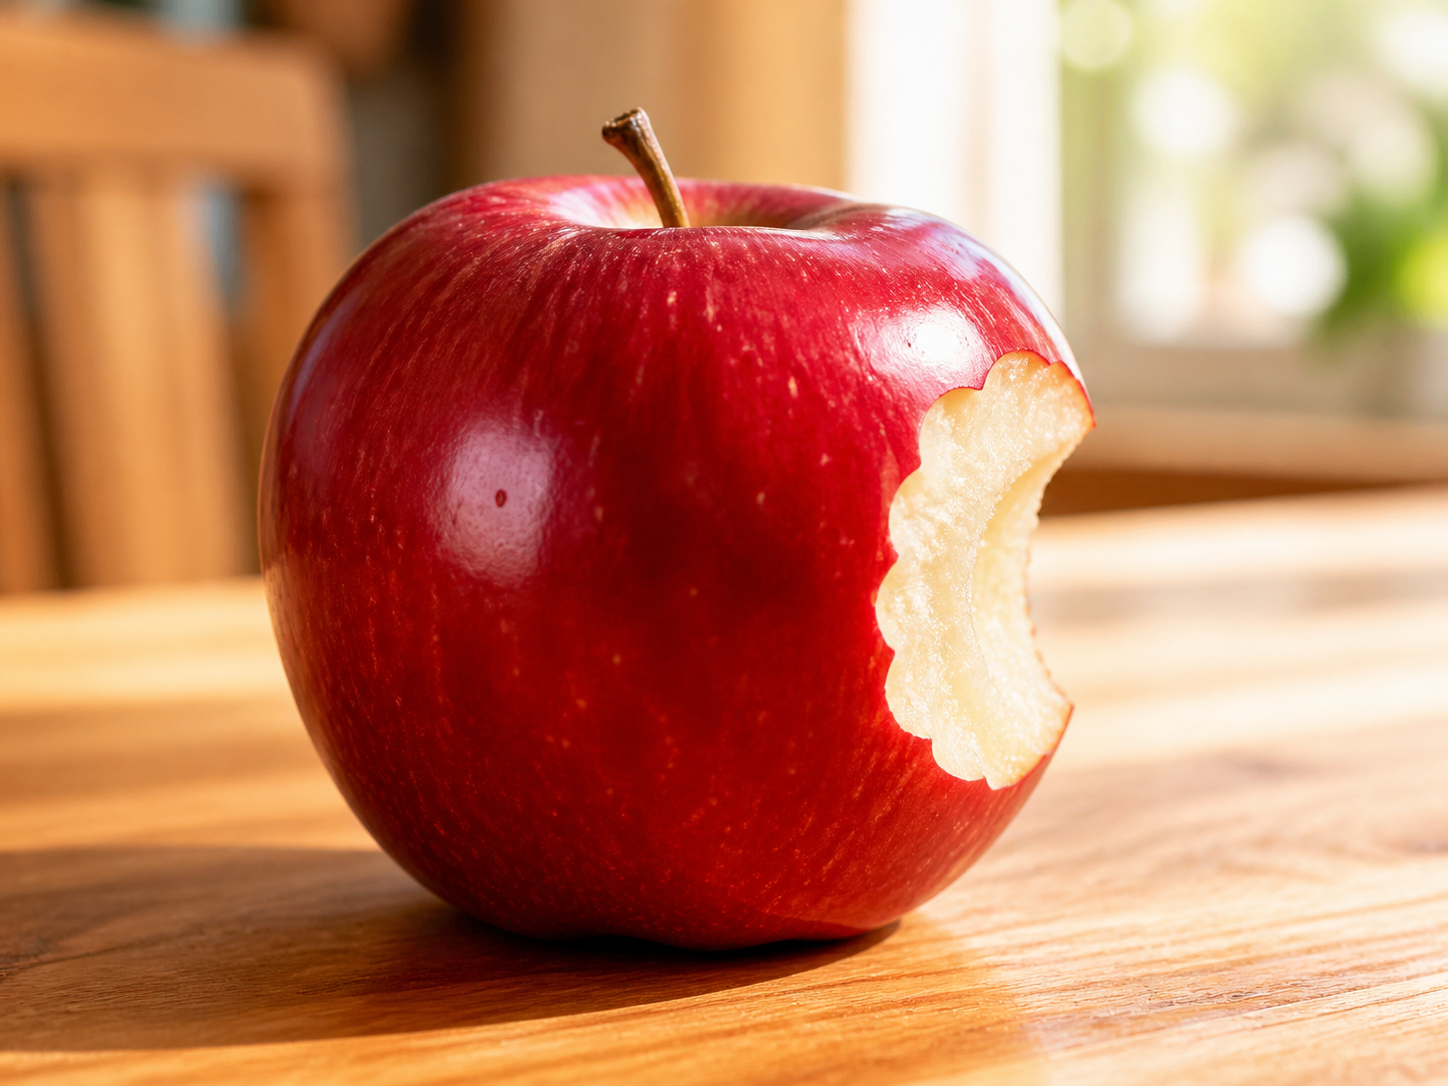
\includegraphics[width=0.52\linewidth]{images/book1/ai/g1-five-senses-apple.png}

{\small Uma maçã para os cinco sentidos: os olhos veem o vermelho dela, a mão sente a casca lisa, os ouvidos escutaram o estalo da mordida que falta, o nariz sente o perfume, a língua guarda o gosto.}
\end{omfigure}

\begin{example}[Experimente: o passeio dos sons]\label{ex:g1:five-senses:sounds}
Sente-se quietinho, feche os olhos e conte os sons ao seu redor
durante um tempinho: um carro, uma voz, o vento, a sua própria
respiração. De olhos fechados, os ouvidos percebem sons que os olhos,
ocupados, faziam você perder. Quase todo mundo encontra $4$ ou $5$
sons que não tinha notado antes.
\end{example}

\begin{remark}[Sentidos que nos protegem]\label{rem:g1:five-senses:danger}
Os sentidos também são guardas. O nariz sente a fumaça antes de os
olhos verem o fogo; a pele puxa a mão de volta da panela quente; um
gosto amargo avisa ``não engula isto''. Nunca prove nem cheire de
propósito uma coisa desconhecida: pergunte antes a um adulto. Os
guardas trabalham melhor quando cuidamos bem deles.
\end{remark}

\section{Observar com cuidado}

Olhar ainda não é \omterm{def:g1:five-senses:observation}{observar}. Todo mundo já \emph{viu} uma joaninha;
quem sabe dizer quantas patas ela tem?

\begin{definition}[Observação]\label{def:g1:five-senses:observation}
\emph{Observar}\index{observar} é usar os sentidos com cuidado, de
propósito, para responder a uma pergunta --- e depois contar ou
desenhar exatamente o que foi percebido, e não o que se esperava. Uma
\emph{observação}\index{observação} é aquilo que o olhar atento
descobriu.
\end{definition}

\begin{method}[Como observar]\label{met:g1:five-senses:how}
\begin{enumerate}
  \item Escolha uma pergunta: \emph{quantas patas tem a joaninha?}
  \item olhe (ou escute, ou toque) devagar, sem pressa;
  \item diga o que percebeu com palavras precisas: não ``é pequena'',
        mas ``é menor que a minha unha'';
  \item desenhe ou conte, para que outra pessoa possa conferir.
\end{enumerate}
Uma boa \omterm{def:g1:five-senses:observation}{observação} pode ser conferida por um colega: se os dois
olharem, os dois devem encontrar $6$ patas.
\end{method}

\begin{example}[Palavras precisas]\label{ex:g1:five-senses:words}
Compare ``a pedra é bonitinha'' com ``a pedra é cinza, lisa, redonda
e mais fria que a minha mão''. A segunda frase é uma
\omterm{def:g1:five-senses:observation}{observação}: outra criança consegue achar essa pedra dentro de
um cesto inteiro.
\end{example}

\begin{omfigure}
\begin{tikzpicture}[scale=0.8]
  % six legs, three per side
  \draw[thick] (1.32,-0.45) -- ++(-30:0.45);
  \draw[thick] (0.9,-0.76) -- ++(-55:0.45);
  \draw[thick] (0.38,-0.92) -- ++(-75:0.45);
  \draw[thick] (-1.32,-0.45) -- ++(210:0.45);
  \draw[thick] (-0.9,-0.76) -- ++(235:0.45);
  \draw[thick] (-0.38,-0.92) -- ++(255:0.45);
  % body, wing split, spots
  \draw[thick, fill=omDef!12] (0,0) ellipse (1.5 and 0.95);
  \draw[thick, omDef] (0,0.95) -- (0,-0.95);
  \fill[omThm] (-0.55,0.3) circle (0.13);
  \fill[omThm] (-0.85,-0.25) circle (0.13);
  \fill[omThm] (0.5,0.4) circle (0.13);
  \fill[omThm] (0.75,-0.25) circle (0.13);
  % head and antennae
  \fill[omDef] (1.55,0) circle (0.3);
  \draw[thick] (1.75,0.18) .. controls (2.0,0.35) .. (2.1,0.55);
  \draw[thick] (1.78,-0.14) .. controls (2.05,-0.28) .. (2.18,-0.42);
  \node[right, font=\small] at (2.8,0.5)
    {Quantas pintas? Quantas patas?};
  \node[right, font=\small] at (2.8,-0.5)
    {Olhe devagar e depois conte.};
\end{tikzpicture}

{\small Observando uma joaninha: olhos atentos contam $4$ pintas
nesta aqui --- e sempre $6$ patas.}
\end{omfigure}

\section{Quando os sentidos se enganam}

Os sentidos são maravilhosos, mas dá para enganá-los. É exatamente
por isso que, nos capítulos que vêm, vamos aprender a \emph{medir}.

\begin{example}[Duas linhas]\label{ex:g1:five-senses:lines}
No desenho abaixo, qual linha é mais comprida? Quase todo mundo
responde ``a de cima''. Agora confira com um pedaço de barbante: as
duas linhas são exatamente do mesmo tamanho. Os olhos se enganaram
por causa das pontas de flecha.
\end{example}

\begin{omfigure}
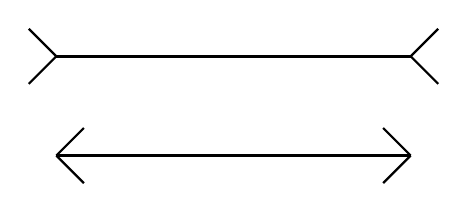
\begin{tikzpicture}[scale=0.9]
  \draw[very thick] (0,1.4) -- (5,1.4);
  \draw[thick] (0,1.4) -- ++(135:0.55) (0,1.4) -- ++(-135:0.55);
  \draw[thick] (5,1.4) -- ++(45:0.55) (5,1.4) -- ++(-45:0.55);
  \draw[very thick] (0,0) -- (5,0);
  \draw[thick] (0,0) -- ++(45:0.55) (0,0) -- ++(-45:0.55);
  \draw[thick] (5,0) -- ++(135:0.55) (5,0) -- ++(-135:0.55);
\end{tikzpicture}

{\small O famoso truque das pontas de flecha: as duas linhas têm o
mesmo comprimento. Confira com um barbante!}
\end{omfigure}

\begin{example}[Experimente: três tigelas]\label{ex:g1:five-senses:bowls}
Peça a um adulto que prepare três tigelas de água: uma fria, uma
morna e uma bem quentinha (mas sem queimar). Deixe uma das mãos na
tigela fria e a outra na tigela quente enquanto conta devagar até
$20$. Depois ponha as duas mãos juntas na tigela do meio: a mesma
água parece quente para uma das mãos e fria para a outra! Só o tato
não é de confiança para dizer o que é quente e o que é frio --- o
próximo capítulo pega exatamente esse problema.
\end{example}

\begin{remark}[Ajudantes dos sentidos]\label{rem:g1:five-senses:tools}
As pessoas constroem ferramentas que ajudam os sentidos: os óculos e
a lupa ajudam os olhos, o estetoscópio do médico ajuda os ouvidos.
Mais adiante neste livro, umas ferramentas chamadas
\emph{instrumentos} vão fazer melhor ainda: elas vão transformar
olhar e tocar em contar e medir, e contar é muito mais difícil de
enganar.
\end{remark}

\section{Exercícios}

\begin{exercise}[$\star$]\label{exo:g1:five-senses:1}
Diga os cinco sentidos e, para cada um, a parte do corpo que faz o
trabalho.
\end{exercise}

\begin{exercise}[$\star$]\label{exo:g1:five-senses:2}
Qual sentido avisa você: (a) que o rádio está ligado? (b) que a sopa
está salgada demais? (c) que o seu casaco está coçando? (d) que as
luzes apagaram?
\end{exercise}

\begin{exercise}[$\star$]\label{exo:g1:five-senses:3}
Um bolo está assando no forno, com a porta fechada, em outro cômodo.
Qual sentido descobre o bolo primeiro? Quais sentidos você vai usar
quando finalmente ganhar uma fatia?
\end{exercise}

\begin{exercise}[$\star$]\label{exo:g1:five-senses:4}
Faça o passeio dos sons do \cref{ex:g1:five-senses:sounds}: de olhos
fechados, conte os sons ao seu redor. Quantos você escutou? Qual
deles surpreendeu você?
\end{exercise}

\begin{exercise}[$\star$]\label{exo:g1:five-senses:5}
Dê uma \omterm{def:g1:five-senses:observation}{observação} do seu sapato usando três palavras precisas,
como no \cref{ex:g1:five-senses:words}. ``Bonito'' e ``legal'' não
valem!
\end{exercise}

\begin{exercise}[$\star$]\label{exo:g1:five-senses:6}
Ana diz: ``O gato é macio.'' Bob diz: ``O gato é o melhor gato do
mundo.'' Qual das frases é uma \omterm{def:g1:five-senses:observation}{observação}, e qual sentido a fez? E
a outra frase, o que é?
\end{exercise}

\begin{exercise}[$\star$]\label{exo:g1:five-senses:7}
Qual sentido avisa você de cada perigo: (a) fumaça em algum lugar da
casa; (b) uma panela quente demais para segurar; (c) um carro vindo
por trás de você?
\end{exercise}

\begin{exercise}[$\star$]\label{exo:g1:five-senses:8}
Um colega fecha os olhos. Você põe na frente dele uma colher, uma
esponja e uma pedrinha, um objeto de cada vez. Ele consegue dizer o
nome dos três só pelo tato? Qual foi o mais fácil de reconhecer?
\end{exercise}

\begin{exercise}[$\star\star$]\label{exo:g1:five-senses:9}
Olhe as duas linhas do \cref{ex:g1:five-senses:lines}. Explique a um
colega como descobrir com certeza qual linha é mais comprida, sem
confiar nos olhos. O seu método também serve para comparar uma linha
com um barbante todo torto?
\end{exercise}
